\section{From guarded hMSC to pure LTS\label{section:deductive-glts-to-lts}}

This section details algorithms to explicitely capture the traces of a guarded hMSC through a pure LTS. Section \ref{subsection:from-ghmsc-to-glts} provides an algorithm to rewrite a g-hMSC to a g-LTS. Section \ref{subsection:from-glts-to-lts} then shows how such g-LTS can be converted to a LTS accepting the same set of traces.

\subsection{From guarded hMSC to guarded LTS\label{subsection:from-ghmsc-to-glts}}

A guarded hMSC can be rewritten as a g-LTS. The latter abstracts from the agents and captures the set of global behaviors covered by the g-hMSC. The rewriting algorithm extends the technique presented in Section \ref{subsection:background-hmsc} that synthesizes a LTS capturing the traces of hMSC \cite{Uchitel:2004}. The algorithm may
be outlined as detailed below. It is illustrated in Fig.~\ref{image:scheduler-ghmsc-glts} for the guarded hMSC in Fig.~\ref{image:scheduler-ghmsc}.

\begin{description}
\item[Handling nodes] Every hMSC node yields a behaviorally equivalent sub-LTS.
\begin{itemize}
\item A MSC node is rewritten as a sub-LTS collecting the linear event sequences from the scenario. For a MSC $M$, the LTS captures the set of traces $\mathcal{L}_{total}(M)$ defined in Section \ref{subsection:background-positive-scenarios}.
\item For a node expanded into a finer-grained hMSC, the procedure is applied recursively to obtain the corresponding sub-LTS.
\item A decision node is rewritten as a sub-LTS having only one state and no event; the same applies to the start and end nodes of the hMSC.
\end{itemize}
In the first two cases, the $Task_{start}$ and $Task_{end}$ special events are added to the corresponding sub-LTS.
\item[Handling edges] The edges in a guarded hMSC yield transitions between the terminal and initial states of the sub-LTS corresponding to their source and target nodes, respectively.
\begin{itemize}
\item An outgoing edge of a decision node is labeled by a guard and yields a guarded transition in the g-LTS.
\item Any other edge is simply converted as a $\tau$ transition.
\end{itemize}
\end{description}

\begin{figure}[H]\centering
\scalebox{0.57}{
  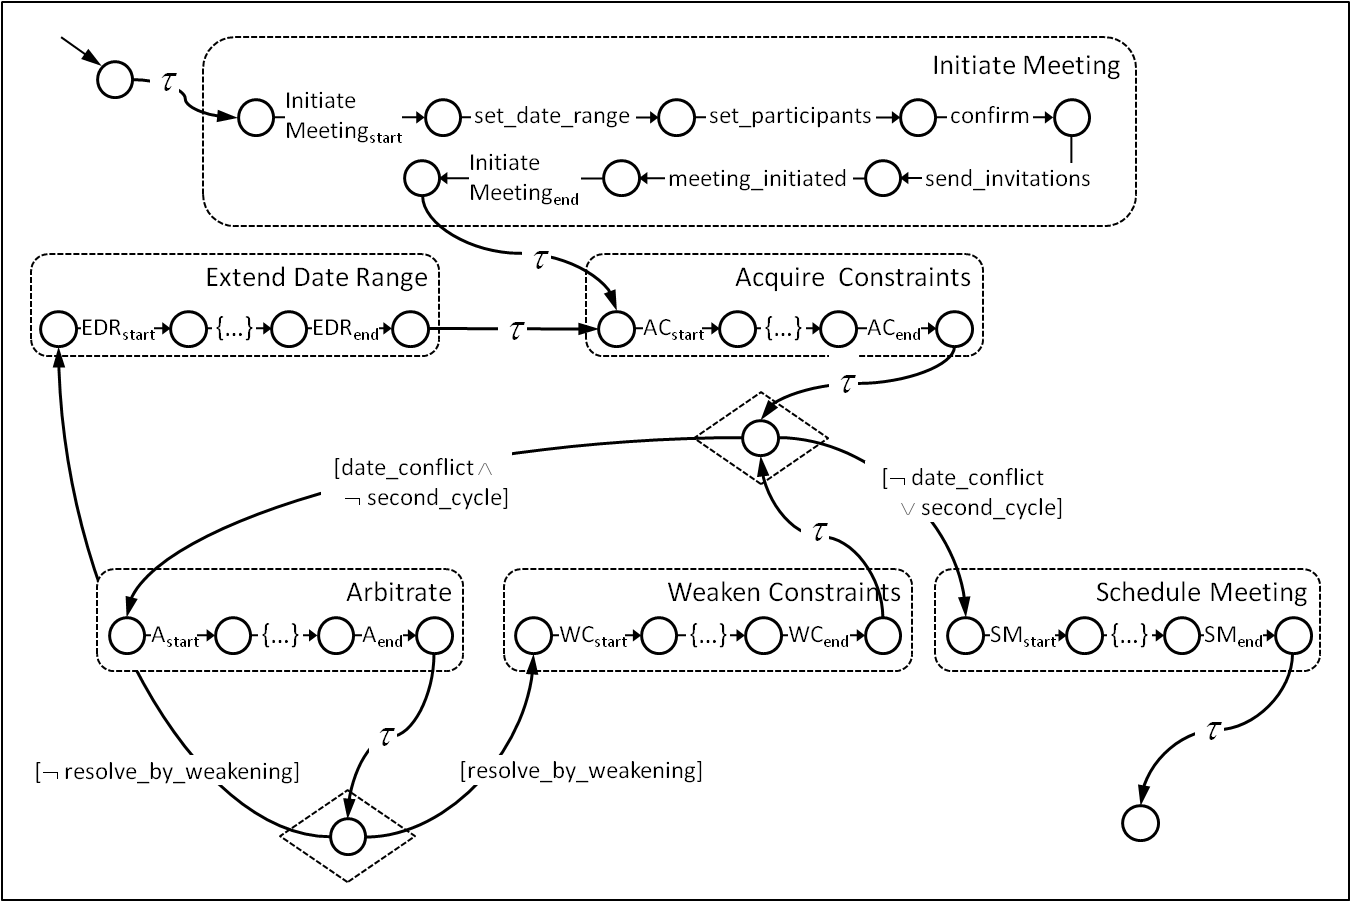
\includegraphics[trim=2mm 2mm 2mm 2mm, clip]{src/3-deductive/images/ghmsc-glts-scheduler}
}
\caption{Rewriting a g-hMSC as a g-LTS, on the meeting scheduler process in Fig.~\ref{image:scheduler-ghmsc}.\label{image:scheduler-ghmsc-glts}}
\end{figure}

\subsection{From guarded LTS to pure LTS\label{subsection:from-glts-to-lts}}

The set of traces accepted by a g-LTS is determined by building a trace-equivalent LTS. For this, a parallel composition of g-LTSs if first computed so as to meet the various acceptance conditions in Section \ref{subsection:glts-trace-semantics}. The first g-LTS in this composition is a super g-LTS meeting the \emph{trace inclusion} and \emph{admissible start} condition. To meet the \emph{guard satisfaction} condition, the set of traces of the super g-LTS is pruned further by composing it with fluent automata. Let us make each of them in the composition further precise.

\noindent \textbf{Super g-LTS} -- By definition, the input g-LTS already meets the \emph{trace inclusion} condition. In order to meet the \emph{admissible start} condition, it is extended by converting the initial condition $C_0$ as an explicit guard from the initial state. 

Let denote the input g-LTS by $G = (Q,\Sigma,\Phi,\delta,q_{0},C_{0})$; the super LTS is defined as:
\begin{equation*}
Super~LTS = (Q \cup \{ q_{start} \}, \Sigma, \Phi, \delta \cup \{(q_{start},C_0,q_0)\},q_{start},true)
\end{equation*}

\noindent \textbf{Fluent g-LTS} -- The \emph{guard satisfaction} condition is enforced by pruning all traces violating guards in the super g-LTS. For this we compose the latter with fluent automata. The latter keep track of the current fluent values; guard events are constrained to happen only when the corresponding guard is true.

A fluent $Fl = \textless Init_{Fl}, Term_{Fl} \textgreater $ yields a g-LTS $G_{Fl} = (Q,\Sigma,\Phi,\delta,q_{0},C_{0})$ where
\begin{align*}
Q      &= \{q_u,q_t,q_f\}            \\
\Sigma &= Init_{Fl} \cup Term_{Fl}   \\
\Phi   &= \{ Fl \} \\
\delta &=    \{~(q_f,e,q_t) \mid e \in Init_{Fl}~\}~\cup \{~(q_t,e,q_t) \mid e \in Init_{Fl}~\} \\
       &\cup~\{~(q_t,e,q_f) \mid e \in Term_{Fl}~\} \cup \{~(q_f,e,q_f) \mid e \in Term_{Fl}~\} \\
       &\cup~\{~(q_u, [Fl], q_t),~(q_u, [\neg Fl], q_f)~\} \\
       &\cup~\{~(q_t, [Fl], q_t),~(q_f, [\neg Fl], q_f)~\} \\
q_0    &= q_u \\
C_0    &= true
\end{align*}

This resulting g-LTS is illustrated in Fig.~\ref{image:fluent-glts} for a generic fluent definition. A transition labeled with a set name between $\{$ and $\}$ brackets is a shortcut denoting one transition for each element of the set.

\begin{figure}[H]\centering
\scalebox{0.75}{
  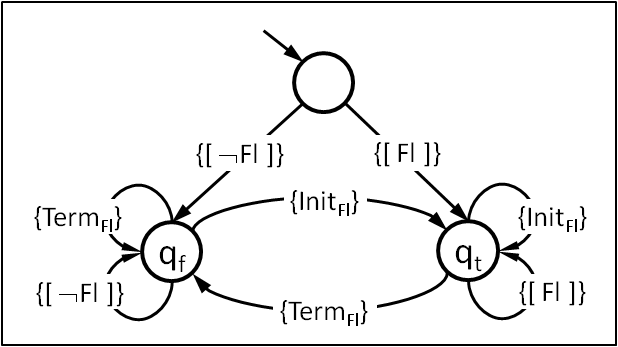
\includegraphics[trim=2mm 2mm 2mm 2mm, clip]{src/3-deductive/images/fluent-glts}
}
\caption{A generic fluent g-LTS\label{image:fluent-glts}}
\end{figure}

For example, consider the following fluent below for the meeting scheduler examplar. The corresponding fluent automaton is shown in Fig.~\ref{image:second-cycle-fluent-glts}.
\begin{center}
fluent $second\_cycle = \textless \{ ExtendDateRange_{end}, \newline WeakenConstraints_{end} \},
 \{ InitiateMeeting_{end} \} \textgreater $\\
\end{center}

\begin{figure}[H]\centering
\scalebox{0.75}{
  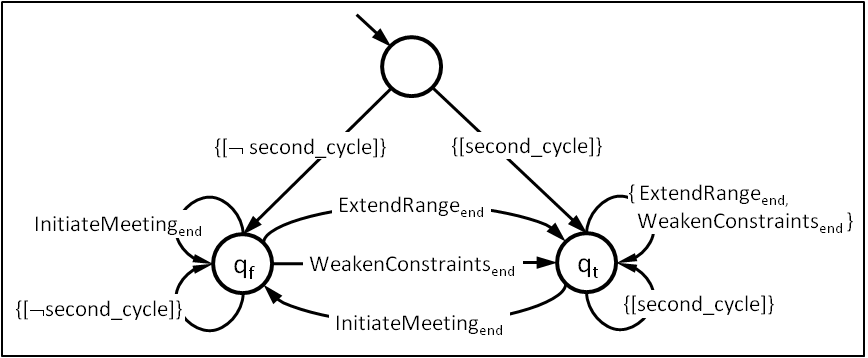
\includegraphics[trim=2mm 2mm 2mm 2mm, clip]{src/3-deductive/images/second-cycle-fluent-glts}
}
\caption{A generic fluent g-LTS\label{image:second-cycle-fluent-glts}}
\end{figure}

\noindent \textbf{Synthesized LTS} -- Putting pieces together, the trace-equivalent LTS of a g-LTS is obtained through the following computation:
\begin{align*}
\left((Super~LTS \parallel G_{Fl_1} \parallel \ldots \parallel G_{Fl_n}) \setminus \mathcal{P}(2^\Phi)\right)^\Delta
\end{align*}

That is, a g-LTS is first obtained through the composition of the Super LTS with fluent automata; all guards are then hidden, resulting in a pure LTS which can be further minimized.
